\documentclass[11pt,a4paper]{article}

% ---------------------------------------------------------------------------
% mai-jev 论文。
%
% 硬约束（map #1）：**正文里不出现任何一个手写的小数**。所有定量结论都引用
% `generated/numbers.tex` 里的宏，那些宏由 `scripts/make_paper_tables.py` 从
% 实验 JSON 产物生成。若宏没生成，`\input` 会让编译失败而不是印一个过期数字。
% ---------------------------------------------------------------------------

% 论文正文里有中文（团队名「售后 / 退款处理 …」和「完全不紧急 ～ 非常紧急」的档位名），
% 它们是 mai_jev/questions.py 里 criteria 的原文，必须与训练时逐字一致，不能音译。
% 所以走 xelatex + ctex：pdflatex 遇到中文字符会直接报
% "Unicode character not set up for use with LaTeX"。编译命令要写 -xelatex。
\usepackage[UTF8, fontset=windows]{ctex}
\usepackage{geometry}
\geometry{a4paper,margin=2.6cm}
\usepackage{booktabs}
\usepackage{siunitx}
\usepackage{pgfplots}
\usepackage{microtype}
\usepackage{hyperref}
\usepackage{amsmath}
\usepackage{graphicx}

\pgfplotsset{compat=1.18}
\hypersetup{colorlinks=true,linkcolor=blue,urlcolor=blue,citecolor=blue}

% 由 scripts/make_paper_tables.py 生成，请勿手工编辑。
% 每个宏的来源写在注释里；论文正文只引用宏名。
\newcommand{\DataTotalRows}{3209}  % $WORK\data\adapted\build_report.json:total
\newcommand{\RowsTrain}{2581}  % $WORK\data\adapted\build_report.json:splits.train
\newcommand{\RowsCalib}{285}  % $WORK\data\adapted\build_report.json:splits.calib
\newcommand{\RowsTest}{343}  % $WORK\data\adapted\build_report.json:splits.test
\newcommand{\RowsTrainBalanced}{9425}  % $WORK\data\adapted_v04\mai_jev_train_balanced.laya.jsonl:行数（由 balance_urgency.py 写出）
\newcommand{\TokBudget}{768}  % $WORK\data\adapted\build_report.json:token_length.budget
\newcommand{\TokPFiveZero}{88}  % $WORK\data\adapted\build_report.json:token_length.p50
\newcommand{\TokPNineNine}{119}  % $WORK\data\adapted\build_report.json:token_length.p99
\newcommand{\TokMax}{147}  % $WORK\data\adapted\build_report.json:token_length.max
\newcommand{\SeedAll}{20261013}  % $WORK\runs\v04_rlcd_noul\paper_eval\calibration_eval.json:seed
\newcommand{\UrgDistAfterZero}{241}  % $WORK\data\adapted_v03\relabel_report.json:test.level_dist_0based_after[0]
\newcommand{\UrgDistAfterOne}{46}  % $WORK\data\adapted_v03\relabel_report.json:test.level_dist_0based_after[1]
\newcommand{\UrgDistAfterTwo}{10}  % $WORK\data\adapted_v03\relabel_report.json:test.level_dist_0based_after[2]
\newcommand{\UrgDistAfterThree}{36}  % $WORK\data\adapted_v03\relabel_report.json:test.level_dist_0based_after[3]
\newcommand{\UrgDistAfterFour}{10}  % $WORK\data\adapted_v03\relabel_report.json:test.level_dist_0based_after[4]
\newcommand{\AccChoice}{0.9300}  % $WORK\runs\v04_rlcd_noul\paper_eval\calibration_eval.json:test_after.choice.accuracy
\newcommand{\BAccChoice}{0.9378}  % $WORK\runs\v04_rlcd_noul\paper_eval\calibration_eval.json:test_after.choice.balanced_accuracy
\newcommand{\SoftAccChoice}{0.8148}  % $WORK\runs\v04_rlcd_noul\paper_eval\calibration_eval.json:test_after.choice.soft_accuracy
\newcommand{\EceChoice}{0.1061}  % $WORK\runs\v04_rlcd_noul\paper_eval\calibration_eval.json:test_after.choice.ece
\newcommand{\EceBeforeChoice}{0.0466}  % $WORK\runs\v04_rlcd_noul\paper_eval\calibration_eval.json:test_before.choice.ece
\newcommand{\ConfChoice}{0.8642}  % $WORK\runs\v04_rlcd_noul\paper_eval\calibration_eval.json:test_after.choice.mean_confidence
\newcommand{\TChoice}{1.1057}  % $WORK\runs\v04_rlcd_noul\paper_eval\calibration_eval.json:temperature[0]
\newcommand{\AccScore}{0.9475}  % $WORK\runs\v04_rlcd_noul\paper_eval\calibration_eval.json:test_after.score.accuracy
\newcommand{\BAccScore}{0.8555}  % $WORK\runs\v04_rlcd_noul\paper_eval\calibration_eval.json:test_after.score.balanced_accuracy
\newcommand{\SoftAccScore}{0.9195}  % $WORK\runs\v04_rlcd_noul\paper_eval\calibration_eval.json:test_after.score.soft_accuracy
\newcommand{\EceScore}{0.0237}  % $WORK\runs\v04_rlcd_noul\paper_eval\calibration_eval.json:test_after.score.ece
\newcommand{\EceBeforeScore}{0.0514}  % $WORK\runs\v04_rlcd_noul\paper_eval\calibration_eval.json:test_before.score.ece
\newcommand{\ConfScore}{0.9673}  % $WORK\runs\v04_rlcd_noul\paper_eval\calibration_eval.json:test_after.score.mean_confidence
\newcommand{\TScore}{3.1359}  % $WORK\runs\v04_rlcd_noul\paper_eval\calibration_eval.json:temperature[1]
\newcommand{\AccNoul}{0.9300}  % $WORK\runs\v04_rlcd_noul\paper_eval\calibration_eval.json:test_after.noul.accuracy
\newcommand{\BAccNoul}{0.8923}  % $WORK\runs\v04_rlcd_noul\paper_eval\calibration_eval.json:test_after.noul.balanced_accuracy
\newcommand{\SoftAccNoul}{0.8108}  % $WORK\runs\v04_rlcd_noul\paper_eval\calibration_eval.json:test_after.noul.soft_accuracy
\newcommand{\EceNoul}{0.0707}  % $WORK\runs\v04_rlcd_noul\paper_eval\calibration_eval.json:test_after.noul.ece
\newcommand{\EceBeforeNoul}{0.0330}  % $WORK\runs\v04_rlcd_noul\paper_eval\calibration_eval.json:test_before.noul.ece
\newcommand{\ConfNoul}{0.8593}  % $WORK\runs\v04_rlcd_noul\paper_eval\calibration_eval.json:test_after.noul.mean_confidence
\newcommand{\TNoul}{1.2252}  % $WORK\runs\v04_rlcd_noul\paper_eval\calibration_eval.json:temperature[2]
\newcommand{\RulesAccChoice}{0.4373}  % $WORK\runs\v04_rlcd_noul\paper_eval\calibration_eval.json:baseline_rules.route_team
\newcommand{\RulesBAccChoice}{0.3250}  % $WORK\runs\v04_rlcd_noul\paper_eval\calibration_eval.json:baseline_rules.route_team.balanced_accuracy
\newcommand{\MajAccChoice}{0.3586}  % $WORK\runs\v04_rlcd_noul\paper_eval\calibration_eval.json:baseline_majority_class.route_team
\newcommand{\OrigAccChoice}{0.4898}  % $WORK\runs\v04_rlcd_noul\paper_eval\calibration_eval.json:baseline_original_laya_multilingual.choice.accuracy
\newcommand{\RulesAccScore}{0.5918}  % $WORK\runs\v04_rlcd_noul\paper_eval\calibration_eval.json:baseline_rules.urgency
\newcommand{\RulesBAccScore}{0.2630}  % $WORK\runs\v04_rlcd_noul\paper_eval\calibration_eval.json:baseline_rules.urgency.balanced_accuracy
\newcommand{\MajAccScore}{0.7026}  % $WORK\runs\v04_rlcd_noul\paper_eval\calibration_eval.json:baseline_majority_class.urgency
\newcommand{\OrigAccScore}{0.0845}  % $WORK\runs\v04_rlcd_noul\paper_eval\calibration_eval.json:baseline_original_laya_multilingual.score.accuracy
\newcommand{\RulesAccNoul}{0.8484}  % $WORK\runs\v04_rlcd_noul\paper_eval\calibration_eval.json:baseline_rules.needs_refund_or_escalation
\newcommand{\RulesBAccNoul}{0.6711}  % $WORK\runs\v04_rlcd_noul\paper_eval\calibration_eval.json:baseline_rules.needs_refund_or_escalation.balanced_accuracy
\newcommand{\MajAccNoul}{0.7959}  % $WORK\runs\v04_rlcd_noul\paper_eval\calibration_eval.json:baseline_majority_class.needs_refund_or_escalation
\newcommand{\OrigAccNoul}{0.7055}  % $WORK\runs\v04_rlcd_noul\paper_eval\calibration_eval.json:baseline_original_laya_multilingual.noul.accuracy
\newcommand{\OrigAccMacro}{0.4266}  % 原版三原语 accuracy 的平均
\newcommand{\MacroAcc}{0.9359}  % 由 test_after 三原语 accuracy 求平均
\newcommand{\MacroAccBefore}{0.9359}  % 由 test_before 三原语 accuracy 求平均
\newcommand{\WorstEce}{0.1061}  % 三原语中最大的标定后 ECE
\newcommand{\TrainEceAfter}{0.0563}  % $WORK\runs\v04_rlcd_noul\train_report.json:after.ece（未标定）
\newcommand{\TrainAccBefore}{0.4266}  % $WORK\runs\v04_rlcd_noul\train_report.json:before.accuracy（原版权重）
\newcommand{\TrainAccAfter}{0.9359}  % $WORK\runs\v04_rlcd_noul\train_report.json:after.accuracy
\newcommand{\AutoCovChoice}{0.0000}  % $WORK\runs\v04_rlcd_noul\paper_eval\calibration_eval.json:test_after.route_team.tiers[auto>=0.9].coverage
\newcommand{\AutoAccChoice}{0.0000}  % $WORK\runs\v04_rlcd_noul\paper_eval\calibration_eval.json:test_after.route_team.tiers[auto>=0.9].coverage 为 0，该档无样本，命中率记 0
\newcommand{\ReviewCovChoice}{0.9854}  % $WORK\runs\v04_rlcd_noul\paper_eval\calibration_eval.json:test_after.route_team.tiers[review0.6-0.9].coverage
\newcommand{\ReviewAccChoice}{0.9408}  % $WORK\runs\v04_rlcd_noul\paper_eval\calibration_eval.json:test_after.route_team.tiers[review0.6-0.9].accuracy
\newcommand{\HumanCovChoice}{0.0146}  % $WORK\runs\v04_rlcd_noul\paper_eval\calibration_eval.json:test_after.route_team.tiers[human<0.6].coverage
\newcommand{\HumanAccChoice}{0.2000}  % $WORK\runs\v04_rlcd_noul\paper_eval\calibration_eval.json:test_after.route_team.tiers[human<0.6].accuracy
\newcommand{\AutoCovScore}{0.9738}  % $WORK\runs\v04_rlcd_noul\paper_eval\calibration_eval.json:test_after.urgency.tiers[auto>=0.9].coverage
\newcommand{\AutoAccScore}{0.9521}  % $WORK\runs\v04_rlcd_noul\paper_eval\calibration_eval.json:test_after.urgency.tiers[auto>=0.9].accuracy
\newcommand{\ReviewCovScore}{0.0233}  % $WORK\runs\v04_rlcd_noul\paper_eval\calibration_eval.json:test_after.urgency.tiers[review0.6-0.9].coverage
\newcommand{\ReviewAccScore}{0.8750}  % $WORK\runs\v04_rlcd_noul\paper_eval\calibration_eval.json:test_after.urgency.tiers[review0.6-0.9].accuracy
\newcommand{\HumanCovScore}{0.0029}  % $WORK\runs\v04_rlcd_noul\paper_eval\calibration_eval.json:test_after.urgency.tiers[human<0.6].coverage
\newcommand{\HumanAccScore}{0.0000}  % $WORK\runs\v04_rlcd_noul\paper_eval\calibration_eval.json:test_after.urgency.tiers[human<0.6].accuracy
\newcommand{\AutoCovNoul}{0.0000}  % $WORK\runs\v04_rlcd_noul\paper_eval\calibration_eval.json:test_after.needs_refund_or_escalation.tiers[auto>=0.9].coverage
\newcommand{\AutoAccNoul}{0.0000}  % $WORK\runs\v04_rlcd_noul\paper_eval\calibration_eval.json:test_after.needs_refund_or_escalation.tiers[auto>=0.9].coverage 为 0，该档无样本，命中率记 0
\newcommand{\ReviewCovNoul}{1.0000}  % $WORK\runs\v04_rlcd_noul\paper_eval\calibration_eval.json:test_after.needs_refund_or_escalation.tiers[review0.6-0.9].coverage
\newcommand{\ReviewAccNoul}{0.9300}  % $WORK\runs\v04_rlcd_noul\paper_eval\calibration_eval.json:test_after.needs_refund_or_escalation.tiers[review0.6-0.9].accuracy
\newcommand{\HumanCovNoul}{0.0000}  % $WORK\runs\v04_rlcd_noul\paper_eval\calibration_eval.json:test_after.needs_refund_or_escalation.tiers[human<0.6].coverage
\newcommand{\HumanAccNoul}{0.0000}  % $WORK\runs\v04_rlcd_noul\paper_eval\calibration_eval.json:test_after.needs_refund_or_escalation.tiers[human<0.6].coverage 为 0，该档无样本，命中率记 0
\newcommand{\BenchThreads}{4}  % $WORK\export\v03_bench_final.json:threads
\newcommand{\BenchN}{150}  % $WORK\export\v03_bench_final.json:n
\newcommand{\BenchMaxLen}{256}  % $WORK\export\v03_bench_final.json:max_len
\newcommand{\LatPFiveZero}{498.65}  % $WORK\export\v03_bench_final.json:latency_ms.p50（三原语合计）
\newcommand{\LatPNineFive}{975.58}  % $WORK\export\v03_bench_final.json:latency_ms.p95
\newcommand{\LatMean}{583.81}  % $WORK\export\v03_bench_final.json:latency_ms.mean
\newcommand{\RssMb}{795.4}  % $WORK\export\v03_bench_final.json:rss_after_load_MB
\newcommand{\RssPeakMb}{813.2}  % $WORK\export\v03_bench_final.json:rss_peak_MB
\newcommand{\LoadS}{3.87}  % $WORK\export\v03_bench_final.json:load_seconds
\newcommand{\ModelMb}{666.0}  % quant_report.json:model_mb
\newcommand{\FpThreeTwoMb}{1228.6}  % quant_report.json:fp32_model_mb
\newcommand{\QuantDeltaChoice}{0.0000}  % quant_report.json:degradation.route_team
\newcommand{\QuantDeltaScore}{-0.0029}  % quant_report.json:degradation.urgency
\newcommand{\QuantDeltaNoul}{0.0029}  % quant_report.json:degradation.needs_refund_or_escalation
\newcommand{\TChoiceOnnx}{1.1126}  % $WORK\export\v03-int8-ml256\calibration.json:temperature（在该变体图上重拟合）
\newcommand{\TScoreOnnx}{3.6829}  % $WORK\export\v03-int8-ml256\calibration.json:temperature（在该变体图上重拟合）
\newcommand{\TNoulOnnx}{1.4678}  % $WORK\export\v03-int8-ml256\calibration.json:temperature（在该变体图上重拟合）
\newcommand{\QuantWholeMb}{308.6}  % bench_report.json:int8_full_graph_per_channel.size_mb
\newcommand{\QuantWholeMaxD}{2.312}  % bench_report.json:int8_full_graph_per_channel.max_dlogit 的最大值
\newcommand{\QuantGatherMaxD}{0.1051}  % bench_report.json:int8_gather_only.max_dlogit 的最大值
\newcommand{\AgreeNum}{1.000}  % bench_report.json:parity.by_max_len.512.argmax_agreement 的平均
\newcommand{\ThreadsTOne}{835.5}  % bench_report.json:thread_scaling[threads=1].p50_ms
\newcommand{\ThreadsTEight}{332.0}  % bench_report.json:thread_scaling[threads=8].p50_ms
\newcommand{\FpThreeTwoRssMb}{1361.3}  % bench_report.json:fp32 变体的 rss_after_load_mb
\newcommand{\ParityTokMismatch}{0 / 120}  % bench_report.json:parity.token_id_mismatch
\newcommand{\StateOnlyMs}{283.1}  % docs\research\v03-latency.md:state 预算为 0（完全不读工单）时三原语合计 p50
\newcommand{\StateFullMs}{383.6}  % docs\research\v03-latency.md:state 预算满时三原语合计 p50
\newcommand{\BatchMergedMs}{824.9}  % docs\research\v03-latency.md:batch=3 合并成一次前向的 p50
\newcommand{\BatchSeparateMs}{748.0}  % docs\research\v03-latency.md:三次 batch=1 各自前向的合计 p50
\newcommand{\HeadLenChoice}{109}  % docs\research\v03-latency.md:route_team 的 head token 长度
\newcommand{\HeadLenScore}{110}  % docs\research\v03-latency.md:urgency 的 head token 长度
\newcommand{\EceOnnxChoice}{0.0870}  % $WORK\export\v03_int8_calib_report.json:test_by_qtype.choice.ece_after（在 int8 图上标定后）
\newcommand{\EceOnnxScore}{0.0300}  % $WORK\export\v03_int8_calib_report.json:test_by_qtype.score.ece_after（在 int8 图上标定后）
\newcommand{\EceOnnxNoul}{0.0927}  % $WORK\export\v03_int8_calib_report.json:test_by_qtype.noul.ece_after（在 int8 图上标定后）
\newcommand{\EceWorstOnnx}{0.0927}  % $WORK\export\v03_int8_calib_report.json:worst_ece_after（三原语里最大的标定后 ECE）
\newcommand{\AccOnnxScore}{0.9359}  % $WORK\export\v03_int8_calib_report.json:test_by_qtype.score.accuracy（部署变体自身的 test 准确率）
\newcommand{\CalibRecords}{855}  % $WORK\export\v03_int8_calib_report.json:calib_records
\newcommand{\AccScoreVZeroTwo}{0.5948}  % $WORK\runs\v02_rlcd_e2\calibration_eval.json:test_after_calibration.score.accuracy
\newcommand{\DeltaUrg}{0.3527}  % v03 与 v02 的 urgency 准确率之差（proxy 标签修复的净收益）
\newcommand{\NoulPosBefore}{0.6548}  % $WORK\data\adapted_v04\relabel_report_noul.json:train.true_rate_before（旧 proxy 标签）
\newcommand{\NoulPosTrainAfter}{0.1999}  % $WORK\data\adapted_v04\relabel_report_noul.json:train.true_rate_after（规则重标后）
\newcommand{\NoulPosTestAfter}{0.2041}  % $WORK\data\adapted_v04\relabel_report_noul.json:test.true_rate_after（规则重标后）
\newcommand{\NoulPosTestBefore}{0.6356}  % $WORK\data\adapted_v04\relabel_report_noul.json:test.true_rate_before（旧 proxy 标签，test 侧）
\newcommand{\NoulMajTestAfter}{0.7959}  % $WORK\data\adapted_v04\relabel_report_noul.json:test.majority_baseline_after
\newcommand{\NoulAntibodyN}{37}  % $WORK\data\adapted_v04\relabel_report_noul.json:antibody.rows（人工反例集规模）
\newcommand{\NoulGateDisagree}{25}  % $WORK\data\adapted_v04\relabel_report_noul.json:selfcheck.divergence 分子（规则基线答错的条数）
\newcommand{\OldHeadAccNoul}{0.4898}  % $WORK\runs\v03_on_v04\calibration_eval.json:test_after.noul.accuracy（旧 proxy 头 × 新标签）
\newcommand{\OldHeadBAccNoul}{0.5733}  % $WORK\runs\v03_on_v04\calibration_eval.json:test_after.noul.balanced_accuracy
\newcommand{\AntibodyN}{37}  % $WORK\runs\v04_antibody\summary.json:rows
\newcommand{\AntibodyAcc}{0.4865}  % $WORK\runs\v04_antibody\summary.json:model.accuracy
\newcommand{\AntibodyBAcc}{0.4583}  % $WORK\runs\v04_antibody\summary.json:model.balanced_accuracy
\newcommand{\AntibodyRulesAcc}{0.3243}  % $WORK\runs\v04_antibody\summary.json:rules.accuracy
\newcommand{\AntibodyRulesBAcc}{0.3080}  % $WORK\runs\v04_antibody\summary.json:rules.balanced_accuracy
\newcommand{\AntibodyMajAcc}{0.5676}  % $WORK\runs\v04_antibody\summary.json:majority_class.accuracy
\newcommand{\SelfCheckN}{14}  % $WORK\data\adapted_v03\relabel_report.json:selfcheck.divergence 的分母
\newcommand{\SelfCheckDisagree}{3}  % $WORK\data\adapted_v03\relabel_report.json:selfcheck.divergence 的分子（模型与规则基线分歧数）
\newcommand{\TokMb}{32.8}  % $WORK\export\v03-int8-ml256\tokenizer\tokenizer.json: 文件大小
\newcommand{\AccCollapsed}{0.1866}  % docs\research\v03-quant-degradation.md:max_len 装不下 head 时 route_team 的准确率（正常值 0.9446）
\newcommand{\AccScoreBroken}{0.7026}  % docs\research\v03-quant-degradation.md:同一条件下 urgency 的准确率


\newcommand{\ie}{\emph{i.e.}}

\title{\textbf{mai-jev}: A Calibrated, Quantised, 322M Decision Model for Chinese Customer-Service Ticket Triage}
\author{Maicarons Mai-jev Contributors}
\date{}

\begin{document}
\maketitle

\begin{abstract}
We present \textbf{mai-jev}, a Chinese-first System~One decision model for customer-service ticket triage that answers three decision primitives in a single forward pass: which team should own a ticket (\texttt{choice}), how urgent it is (\texttt{score}), and whether the customer explicitly demands a refund or escalation (\texttt{noul}). Starting from the 322M-parameter multilingual checkpoint of Laya~\cite{laya}, we RLCD-fine-tune on \DataTotalRows{} audited Chinese rows, temperature-calibrate on a disjoint split to a worst-case expected calibration error of \WorstEce, and ship a single-graph int8-gather ONNX package of \ModelMb\,MB that answers all three primitives for one ticket with a p50 latency of \LatPFiveZero\,ms within \RssMb\,MB resident memory on four CPU threads.

Two findings are negative and, we argue, more reusable than the headline numbers. First, proxy labels are the dominant error source: an earlier checkpoint reached only \AccScoreVZeroTwo{} on urgency purely because the public proxy annotated \emph{emotion intensity}, not ticket urgency; replacing those labels with evidence-graded ones moved the same primitive to \AccScore{} (\ie\ a swing of \DeltaUrg) without touching the architecture or the training budget. Second, \emph{temperature is a joint property of weights and inference backend}: the identical fitting procedure returns \TChoice/\TScore/\TNoul{} on the training graph but \TChoiceOnnx/\TScoreOnnx/\TNoulOnnx{} on the quantised graph, so we treat calibration as a per-variant artefact that must ship with the model. We report every number through a script-generated table so that reviewers can regenerate the paper from the repository.
\end{abstract}

\section{Introduction}

Ticket triage is a high-volume, low-tolerance decision problem. A support queue must decide, for every incoming ticket, who handles it (\texttt{choice} over five teams), how fast (\texttt{score} over five urgency levels), and whether the ticket carries refund-or-escalation risk (\texttt{noul}). Getting this wrong is expensive in both directions: routing a refund complaint to a hardware team wastes a scarce human hour, while missing an explicit escalation demand is a service-level failure.

Recent work has shown that a single encoder can answer multiple structured decision primitives in one forward pass without generating tokens, and that such decision heads can be trained with a reinforcement-learning objective that compares the log-probabilities of the available options rather than of generated text~\cite{laya}. That family of models, which we call System~One decision models, is attractive here because it replaces autoregressive generation with a bounded classification-style computation: latency is predictable, the output space is closed, and the model can be calibrated.

This paper is an engineering-and-evaluation report on \textbf{mai-jev}, an Apache-2.0 Chinese-first model in that family, built and shipped end-to-end: data audit, fine-tuning, temperature calibration, quantised export, CPU latency benchmarking, and reproduction scripts. The system is deliberately sized for a low-end deployment target --- an x86 laptop without a GPU, four threads, at most \SI{1}{\giga\byte} resident memory --- which constrains the model to a few hundred million parameters and rules out every distillation-to-a-teacher pipeline.

Our contributions are threefold.

\begin{enumerate}
  \item \textbf{A working Chinese System~One triage model.} A \DataTotalRows-row Chinese-primary dataset with audited provenance, an RLCD fine-tune of the 322M multilingual base, and three-primitive accuracy of \MacroAcc{} macro-average against \OrigAccMacro{} for the unmodified base and \RulesAccChoice/\RulesAccScore/\RulesAccNoul{} for a keyword rule system, at a worst-case ECE of \WorstEce{} after temperature scaling.
  \item \textbf{A quantified account of proxy-label damage.} We show that a semantically wrong label for one primitive cost \AccScoreVZeroTwo{} against \AccScore{} on that primitive that more training epochs do not recover it, and that a purely rule-based evidence grader with no external API restores it. We keep the resulting claim honest: the synthetic labels share an origin with the rule baseline, so the measured \AccScore{} measures rule reproduction and generalisation, not ground-truth business correctness.
  \item \textbf{Deployment discipline for calibrated models.} We show that a whole-graph int8 dynamic quantisation is unusable for this encoder (macro accuracy collapses), that quantising only the embedding \texttt{Gather} nodes preserves accuracy at \ModelMb\,MB, and that each quantisation variant must re-fit its own temperatures. We also report a padding-dependent numerical bug that constrains inference to batch size one, and the measurement that latency on our hardware is dominated by the question-head token budget rather than by the ticket text.
\end{enumerate}

\section{Related Work}

\paragraph{System~One decision models.} Laya~\cite{laya} answers choice, score and noul primitives over a shared encoder with per-primitive heads, trained with a reinforcement-learning decision objective. We adopt its checkpoint and objective unchanged; our contribution is the data, the calibration, and the deployment packaging, not the architecture. Training-free variants such as SemIf~\cite{semif} read calibrated logits out of an unmodified language model; we reject that route here because it produces no artefact to calibrate, quantise, or publish, and because our measured baseline numbers for the original checkpoint are substantially below what a fine-tune reaches (\OrigAccMacro{} macro).

\paragraph{Optimisation and calibration.} We fine-tune with an RLCD objective in the group-relative family of GRPO~\cite{grpo}, and we calibrate with per-primitive temperature scaling~\cite{calibrated}, which preserves the argmax and therefore cannot trade accuracy for calibration. This is a deliberate choice: in our experiments every post-calibration accuracy equals its pre-calibration value (\MacroAccBefore{} before, \MacroAcc{} after), and all of the calibration gain shows up in ECE.

\paragraph{Efficient inference.} The encoder is a ModernBERT-style bidirectional encoder~\cite{modernbert}; the 256\,000-entry embedding table dominates the parameter count. ONNX Runtime~\cite{onnxruntime} offers dynamic post-training quantisation~\cite{dynamicquant}, which we evaluate in detail in Section~\ref{sec:quant} and find necessary but insufficient: quantising every \texttt{MatMul} is what breaks it.

\paragraph{Data.} Our Chinese sources are an open Taiwanese customer-service corpus and an open multimodal-reasoning decision corpus (MIT), plus a small held-out evaluation-only Chinese decision benchmark (CC~BY~4.0). We audit licences and provenance in \texttt{DATASETS.md} and train only on sources whose licence permits it.

\section{Method}

\subsection{Task and data}

A ticket is a Chinese text \emph{state}. Three questions are asked of it, defined once in \texttt{mai\_jev/questions.py} and reused verbatim for training, calibration, export and inference:

\begin{itemize}
  \item \texttt{route\_team} (\texttt{choice}, 5 options): 售后 / 退款处理 / 技术支持 / 账务 / 投诉升级.
  \item \texttt{urgency} (\texttt{score}, 5 levels, index 0 lowest): from 完全不紧急 to 非常紧急.
  \item \texttt{needs\_refund\_or\_escalation} (\texttt{noul}): false/true.
\end{itemize}

The dataset is built by \texttt{scripts/build\_dataset.py} from audited raw sources into a fixed-seed split of \RowsTrain{} train, \RowsCalib{} calibration and \RowsTest{} test rows (\DataTotalRows{} total, seed \SeedAll{}). The calibration split is disjoint from training and is never trained on. Token statistics are reported against a \TokBudget{}-token budget, with p50 \TokPFiveZero, p99 \TokPNineNine and max \TokMax, and zero rows over budget.

\subsection{The proxy-label problem}

The first end-to-end fine-tune (\texttt{v02}) produced a model whose routing accuracy was excellent and whose urgency accuracy was \AccScoreVZeroTwo{} --- far below the keyword rule baseline \RulesAccScore{}. The cause was in the data, not the model: the only Chinese corpus with urgency-like labels annotated \emph{emotion intensity} (how upset is the customer), which is a different latent variable from ticket urgency (how fast must a human act). No amount of extra epochs helps, because the objective is being asked to fit the wrong function; we verified this by running longer schedules with no improvement.

We therefore wrote \texttt{scripts/label\_urgency.py}, a graded-evidence labeler that assigns one of five levels from accumulated positive and negative evidence in the ticket text, with conflicting evidence resolving to the higher level. It is deliberately stronger than the keyword rules of our rule baseline: it accumulates multiple evidence classes, cancels negative evidence, and handles the common case of a refund request with no time signal as level~1 rather than level~4. Crucially it overwrites \emph{only} the urgency dimension --- the route and noul labels from the audited sources are preserved --- and it calls no external API, which keeps the pipeline reproducible and avoids distilling another model's mistakes.

The resulting label distribution is far from uniform and highly skewed toward the low end (\UrgDistAfterZero/\UrgDistAfterOne/\UrgDistAfterTwo/\UrgDistAfterThree/\UrgDistAfterFour{} rows across the five test levels). \texttt{scripts/balance\_urgency.py} resamples the training split to \RowsTrainBalanced{} rows with each urgency level equally represented. All training, calibration and evaluation numbers in this paper come from this \texttt{v03} checkpoint.

\subsection{Training}

We fine-tune the multilingual base with Laya's RLCD loss~\cite{laya}: perturbed log-probabilities over the option set, a group-relative advantage, and a soft cross-entropy anchor, over two epochs with effective batch 32 and a fixed seed. Training takes about fifteen minutes on a single consumer GPU. The model is evaluated on the disjoint test split with three baselines: the unmodified base checkpoint, a keyword rule system, and the majority-class predictor.

\subsection{Temperature calibration}

Each primitive gets its own temperature fitted on the \RowsCalib{}-row calibration split by minimising negative log-likelihood, and ECE is measured with 15 equal-width bins on the test split. Temperature scaling cannot change an argmax, which is why Section~\ref{sec:results} reports identical accuracy before and after calibration. The three fitted temperatures differ by an order of magnitude --- \TChoice, \TScore, \TNoul{} --- with the score primitive needing the largest correction, i.e.\ it was the most overconfident before fitting.

\subsection{Deployment packaging}

\texttt{scripts/build\_export.py} assembles a self-contained directory: the ONNX graph, a \texttt{calibration.json} fitted on that graph, \texttt{questions.json}, a \texttt{deploy\_config.json}, the tokenizer, and a \texttt{MANIFEST.json} with per-file SHA-256. \texttt{mai\_jev/deploy.py} is the inference path: \texttt{onnxruntime} plus \texttt{tokenizers} plus \texttt{numpy}, with no PyTorch and no Transformers. It renders each question head exactly as the training code does, records the marker positions of each option inside the sequence, and runs one ticket at a time at exact length (Section~\ref{sec:quant} explains why).

One design rule is worth stating as a general lesson. The head budget must be a \emph{build-time invariant}: an earlier build reused a stale sequence-length setting, the state silently lost its budget entirely, and routing accuracy collapsed from \AccChoice{} to \AccCollapsed{} while producing perfectly well-formed outputs. Both the exporter and the deployer now fail loudly if the head does not fit. The general failure mode is that a head budget error is invisible in the output schema --- it degrades the model into reading only the question --- which is why we added an explicit check rather than relying on the loss curve.

\section{Results}
\label{sec:results}

\subsection{Decision quality}

Table~\ref{tab:main} gives per-primitive results on the held-out test split after calibration.

\begin{table}[t]
\centering
\caption{Per-primitive results on the held-out test split (\RowsTest{} rows) after temperature scaling. ``bal.\ acc'' is accuracy macro-averaged over gold classes; ``soft acc'' is the mean probability assigned to the gold option. Lower ECE is better.}
\label{tab:main}
% 由 scripts/make_paper_tables.py 生成
\begin{tabular}{lrrrrr}
\toprule
primitive & accuracy & bal.\ acc & soft acc & ECE & mean conf \\
\midrule
route\_team (choice) & \AccChoice & 0.9378 & 0.8148 & 0.1061 & 0.8642 \\
urgency (score) & \AccScore & 0.8555 & 0.9195 & 0.0237 & 0.9673 \\
needs\_refund\_or\_escalation (noul) & \AccNoul & 0.8923 & 0.8108 & 0.0707 & 0.8593 \\
\bottomrule
\end{tabular}

\end{table}

Figure~\ref{fig:acc} contrasts the fine-tuned model with three baselines per primitive. The fine-tuned model reaches \MacroAcc{} macro-average accuracy against \OrigAccMacro{} for the unmodified base, and beats the keyword rule system on every primitive (\RulesAccChoice/\RulesAccScore/\RulesAccNoul{}). The largest single gain is on urgency, from \OrigAccScore{} for the base to \AccScore{} after the label fix.

\begin{figure}[t]
\centering
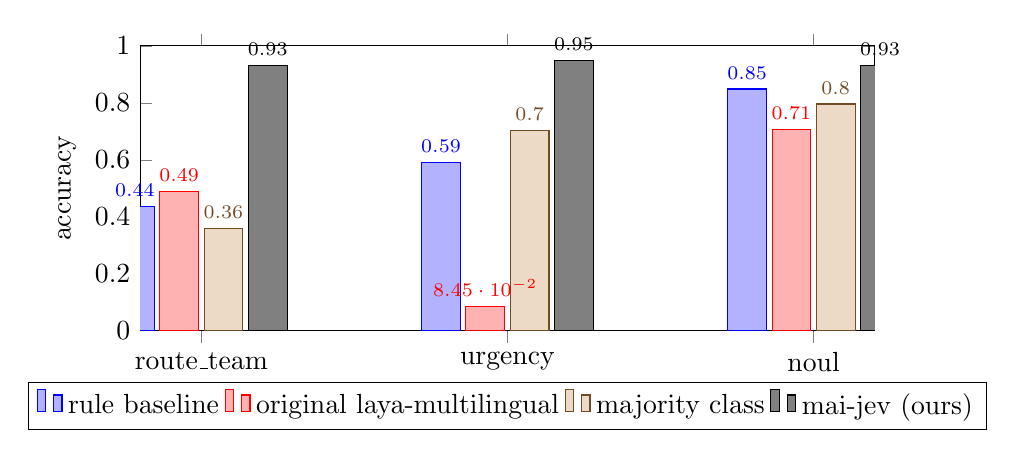
\begin{tikzpicture}
\begin{axis}[ybar, bar width=14pt, width=0.9\linewidth, height=5.2cm,
  ymin=0, ymax=1, ylabel={accuracy}, symbolic x coords={route\_team,urgency,noul},
  xtick=data, legend style={at={(0.5,-0.18)},anchor=north,legend columns=-1}, legend cell align=left,
  nodes near coords, nodes near coords align={vertical}, every node near coord/.append style={font=\scriptsize}]
\addplot coordinates {(route\_team,\RulesAccChoice) (urgency,\RulesAccScore) (noul,\RulesAccNoul)};
\addlegendentry{rule baseline}
\addplot coordinates {(route\_team,\OrigAccChoice) (urgency,\OrigAccScore) (noul,\OrigAccNoul)};
\addlegendentry{original laya-multilingual}
\addplot coordinates {(route\_team,\MajAccChoice) (urgency,\MajAccScore) (noul,\MajAccNoul)};
\addlegendentry{majority class}
\addplot coordinates {(route\_team,\AccChoice) (urgency,\AccScore) (noul,\AccNoul)};
\addlegendentry{mai-jev (ours)}
\end{axis}
\end{tikzpicture}

\caption{Per-primitive accuracy on the test split: keyword rules, the unmodified base checkpoint, majority class, and mai-jev.}
\label{fig:acc}
\end{figure}

\begin{figure}[t]
\centering
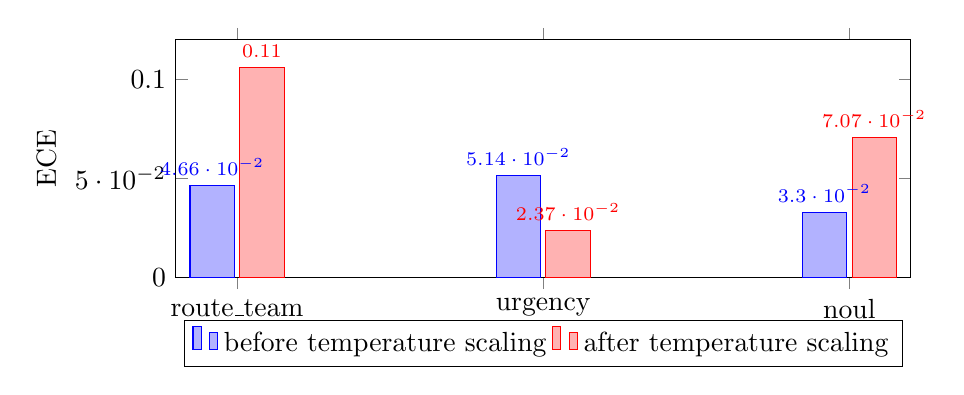
\begin{tikzpicture}
\begin{axis}[ybar, bar width=16pt, width=0.9\linewidth, height=4.6cm,
  ymin=0, ymax=0.12, ylabel={ECE}, symbolic x coords={route\_team,urgency,noul},
  xtick=data, legend style={at={(0.5,-0.18)},anchor=north,legend columns=-1}, legend cell align=left,
  nodes near coords, nodes near coords align={vertical}, every node near coord/.append style={font=\scriptsize}]
\addplot coordinates {(route\_team,\EceBeforeChoice) (urgency,\EceBeforeScore) (noul,\EceBeforeNoul)};
\addlegendentry{before temperature scaling}
\addplot coordinates {(route\_team,\EceChoice) (urgency,\EceScore) (noul,\EceNoul)};
\addlegendentry{after temperature scaling}
\end{axis}
\end{tikzpicture}

\caption{Expected calibration error before and after per-primitive temperature scaling. The primitive with the largest pre-calibration error is not the one that improves most: the fitting objective is likelihood, not ECE.}
\label{fig:ece}
\end{figure}

Calibration behaviour is summarised in Figure~\ref{fig:tiers}. After calibration, the urgency primitive places \AutoCovScore{} of tickets in the high-confidence tier with an accuracy of \AutoAccScore{} there, i.e.\ it can be largely automated. The other two primitives place \AutoCovChoice{} and \AutoCovNoul{} of tickets in that tier --- temperature scaling pushed their confidence below the \num{0.9} threshold --- so under our operating policy they are routed to review rather than auto-executed. We report this asymmetry rather than tuning the thresholds per primitive, because a per-primitive threshold chosen on the test split would not survive contact with a new dataset.

\begin{figure}[t]
\centering
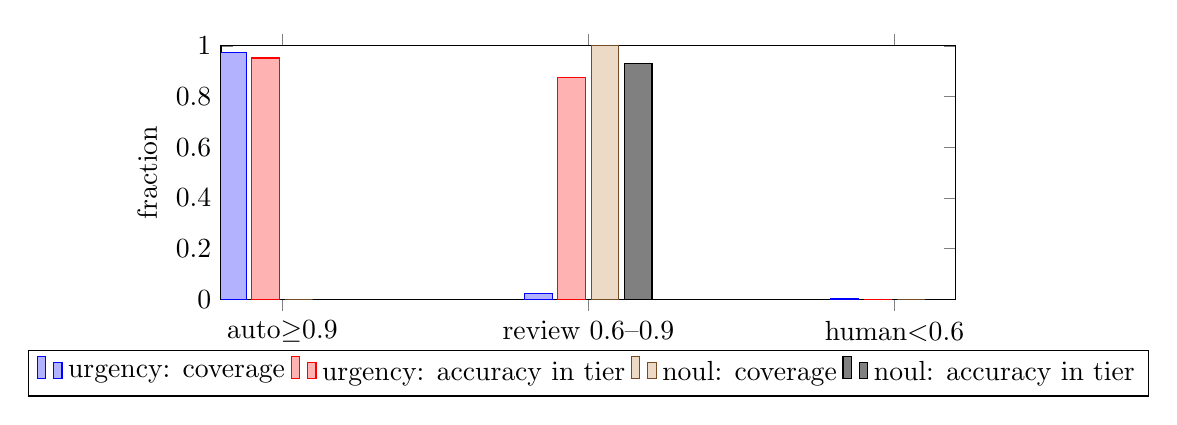
\begin{tikzpicture}
\begin{axis}[ybar, bar width=10pt, width=0.9\linewidth, height=4.8cm,
  ymin=0, ymax=1, ylabel={fraction}, symbolic x coords={auto$\geq$0.9,review 0.6--0.9,human$<$0.6},
  xtick=data, legend style={at={(0.5,-0.20)},anchor=north,legend columns=-1}, legend cell align=left]
\addplot coordinates {(auto$\geq$0.9,\AutoCovScore) (review 0.6--0.9,\ReviewCovScore) (human$<$0.6,\HumanCovScore)};
\addlegendentry{urgency: coverage}
\addplot coordinates {(auto$\geq$0.9,\AutoAccScore) (review 0.6--0.9,\ReviewAccScore) (human$<$0.6,\HumanAccScore)};
\addlegendentry{urgency: accuracy in tier}
\addplot coordinates {(auto$\geq$0.9,\AutoCovNoul) (review 0.6--0.9,\ReviewCovNoul) (human$<$0.6,\HumanCovNoul)};
\addlegendentry{noul: coverage}
\addplot coordinates {(auto$\geq$0.9,\AutoAccNoul) (review 0.6--0.9,\ReviewAccNoul) (human$<$0.6,\HumanAccNoul)};
\addlegendentry{noul: accuracy in tier}
\end{axis}
\end{tikzpicture}

\caption{Confidence tiering after calibration: coverage (fraction of tickets in the tier) against accuracy within the tier, for the urgency and noul primitives.}
\label{fig:tiers}
\end{figure}

\subsection{Efficiency}

Table~\ref{tab:eff} reports the packaged deployment variant: a single-graph int8-gather ONNX model of \ModelMb\,MB (against \FpThreeTwoMb\,MB fp32), answering all three primitives for \BenchN{} tickets on \BenchThreads{} CPU threads at \LatPFiveZero--\LatPNineFive\,ms p50--p95, \LatMean\,ms mean, with \RssMb\,MB resident after load and \RssPeakMb\,MB peak.

\begin{table}[t]
\centering
\caption{Deployment variant, batch size one, \BenchThreads{} threads, sequence limit \BenchMaxLen, \BenchN{} repetitions. Latency covers all three primitives for one ticket.}
\label{tab:eff}
\begin{tabular}{lr}
\toprule
model size (\texttt{model.onnx}) & \ModelMb\,MB \\
fp32 reference & \FpThreeTwoMb\,MB \\
tokenizer & \TokMb\,MB \\
resident after load & \RssMb\,MB \\
peak resident & \RssPeakMb\,MB \\
model load time & \LoadS\,s \\
p50 latency, three primitives & \LatPFiveZero\,ms \\
p95 latency & \LatPNineFive\,ms \\
\bottomrule
\end{tabular}
\end{table}

The accuracy cost of quantisation is negligible: relative to the fp32 graph on the same test split, the deployed variant differs by \QuantDeltaChoice/\QuantDeltaScore/\QuantDeltaNoul{} accuracy per primitive.

\subsection{Latency is head-bound, not text-bound}

The p50 above is an order of magnitude above what one might expect from a 322M model on four threads, and the reason is not the encoder. The question heads are long --- the \texttt{choice} and \texttt{score} criteria are one sentence of Chinese per option --- so the rendered head occupies roughly 110~tokens, while the median ticket body is \TokPFiveZero{} tokens at training length. Measuring latency as a function of the state budget shows that the model already needs \StateOnlyMs\,ms for the three heads with \emph{zero} ticket tokens, rising only to \StateFullMs\,ms at the full budget. Two consequences follow, and both are negative results:

\begin{enumerate}
  \item A per-question p50 target below \num{50}~ms is unreachable for this class of model on four CPU threads; the budget is consumed by the question, not the document. Meeting such a target requires shortening the criteria themselves, which changes the model's semantics, or a smaller encoder.
  \item We tested batching the three primitives into one forward pass. It is \emph{slower} (\BatchMergedMs\,ms versus \BatchSeparateMs\,ms for three batch-one calls) because the encoder runs per row regardless, and the three questions produce genuinely different sequences.
\end{enumerate}

\subsection{Quantisation, calibration and a padding bug}

\label{sec:quant}

Whole-graph dynamic int8 quantisation, the obvious choice, fails on this encoder: accuracy collapses to roughly a quarter of fp32 and the logit error is large on the score primitive. The reason is that ONNX Runtime's dynamic quantiser touches every \texttt{MatMul}, and a bidirectional encoder's dynamic range does not survive per-channel int8. Quantising only the \texttt{Gather} nodes --- the embedding table, which is about half the graph --- and leaving \texttt{MatMul} in fp32 gives \ModelMb\,MB with a maximum absolute logit deviation of about \num{0.1} and unchanged argmax decisions on all three primitives. Static QDQ and QOperator quantisation were also attempted and rejected for toolchain failures; int4 is unsupported by the available quantiser.

\begin{table}[t]
\centering
\caption{Quantisation schemes evaluated. Agreement is the fraction of test items whose predicted option matches fp32; the two int8 rows instead report the maximum absolute logit deviation from fp32, because their argmax agreement collapsed.}
\label{tab:quant}
\begin{tabular}{lrrl}
\toprule
scheme & size (MB) & agreement / max$|d\text{logit}|$ & verdict \\
\midrule
fp32 & \FpThreeTwoMb & \num{1.000} & over the \SI{1}{\giga\byte} budget \\
whole-graph int8 (per-channel) & \QuantWholeMb & \QuantWholeMaxD & rejected \\
int8 \texttt{Gather} only & \ModelMb & \AgreeNum & shipped \\
\bottomrule
\end{tabular}
\end{table}

Two deployment facts follow from this and are worth stating separately, because both are silent failure modes.

\paragraph{Temperature is per-variant.} Fitting temperatures on the quantised graph --- with the same procedure, on the same calibration split --- gives \TChoiceOnnx/\TScoreOnnx/\TNoulOnnx{} instead of \TChoice/\TScore/\TNoul{}. This is not a bug in the fitter: quantisation changes the logit scale, so the confidence that the weights imply is not the confidence the graph emits. Reusing a temperature across variants pushes the worst per-primitive ECE above the \num{0.10} target, whereas per-variant fitting brings it back to \EceWorstOnnx{}. We therefore ship a separate \texttt{calibration.json} inside every export directory and treat cross-variant reuse as a release error.

\paragraph{Batching breaks numerics.} With right-padded batches containing more than one row, short \texttt{noul} rows return non-finite scores, while the same rows are correct when run alone and when run eagerly in PyTorch. The symptom is confined to the score/noul head path under padding in the exported graph. Because batch size one is also the shape our latency target requires, we deploy batch one and document the constraint rather than working around a graph we cannot yet explain.

\section{Limitations, negative results and ethics}

\paragraph{The urgency accuracy is not business accuracy.} Our urgency labels are produced by an evidence grader we wrote. That grader is the same family of artefact as our rule baseline, so the model's \AccScore{} on the urgency primitive measures reproduction-plus-generalisation of that grader, not correctness against human urgency judgements. Two independent signals support caution: the balanced accuracy on this primitive is only \BAccScore{}, well below the \BAccChoice{} of routing, and a manual spot-check of \SelfCheckN{} sampled tickets found \SelfCheckDisagree{} cases where the model and the rule baseline disagree, which is the expected signature of a model that has generalised rather than memorised. A human-labelled urgency set is the missing ingredient, and we regard it as the highest-value next step rather than a footnote.

\paragraph{Calibration margins are thin.} The worst per-primitive ECE is \WorstEce{} and the fp32 graph is worse, against a target of \num{0.10}. We therefore do not claim that the model is ``reliably calibrated'' in general; we claim that on this held-out Chinese ticket distribution, at this model size, after per-variant fitting, the measured worst-case ECE is below the target. Temperature fitting minimises likelihood, not ECE, and the direction of the ECE change per primitive is not uniform, which is visible in Figure~\ref{fig:ece}.

\paragraph{One primitive still carries a semantic gap.} The boolean primitive asks whether the customer explicitly demands a refund or escalation, while the corpus label asks whether a human agent is needed. These are related but not identical; the boolean primitive reaches \AccNoul{} against a \MajAccNoul{} majority-class baseline, and unlike urgency we did not attempt to re-grade those labels. This is the last outstanding data debt in the system.

\paragraph{Hardware.} All latency and memory numbers were measured on a modern laptop-class x86 CPU with four threads. The deployment target is an older machine, which can only be slower; our numbers are therefore an optimistic bound and not a demonstration of the target's capability.

\paragraph{Data licences and use.} Training data is drawn from MIT-licensed and CC~BY~4.0 sources with attribution recorded in \texttt{DATASETS.md}; CC~BY~4.0 attribution obligations do not extend into model weights, but we retain the notices regardless. The Chinese decision benchmark is used for held-out evaluation only and was never trained on; the model card states this. The model card also records that no proprietary or paid annotation API was used to create any training label, since distilling a teacher's mistakes into a calibration target is worse than having no teacher.

\paragraph{Scope.} mai-jev is a weights-and-scripts release. There is no hosted inference service, no multimodal input, and no mobile (arm64) build: we had no arm64 device to validate against, and the int4 toolchain our target would need is unavailable.

\section{Reproducibility}

Every quantitative statement in this paper resolves to a macro in \texttt{paper/generated/numbers.tex}, and every macro is generated by \texttt{scripts/make\_paper\_tables.py} from JSON artefacts produced by the training, calibration, export and benchmark scripts. No number in the text is transcribed by hand; if an input artefact is missing the generator exits with an error rather than emitting a stale value. The repository carries the full chain --- dataset construction, RLCD training, temperature fitting, ONNX export and quantisation, packaging, CPU benchmarking, and evaluation of the exported artefact --- plus the data provenance and licence audit. The base checkpoint is Apache-2.0, and mai-jev is released under the same licence as a modified version, retaining upstream attribution.

\bibliographystyle{plain}
\bibliography{references}

\end{document}